\chapter{Testing and Results}
\label{ch:chapter2}
\ifpdf
    \graphicspath{{Chapter2/Chapter2Figs/PNG/}{Chapter2/Chapter2Figs/PDF/}{Chapter2/Chapter2Figs/}}
\else
    \graphicspath{{Chapter2/Chapter2Figs/EPS/}{Chapter2/Chapter2Figs/}}
\fi

In this chapter the implementation of DMQMC is tested on some small antiferromagnetic bipartite Heisenberg lattices. The benefits of testing on such systems is that they are sign-problem free\cite{Spencer2012} and the ground-state properties have been the subject of extensive study in the literature. All results in this section were simulated in the $M_S=0$ total spin subspace with an inverse-temperature step of $\Delta\beta J = 0.1$ and in the absence of an external magnetic field ($h=0$).

%We begin by studying the properties of the $4\times4$ antiferromagnetic Heisenberg lattice. Next we attempt to apply the method to the $6\times6$ antiferromagnetic Heisenberg lattice. At this point a major flaw in the DMQMC method is discovered and a suitable importance sampling solution is developed. With this new importance sampling method the $6\times6$ antiferromagnetic Heisenberg lattice is revisited as well as the larger $4\times4\times4$ system.

\section{The $4\times4$ antiferromagnetic Heisenberg Lattice}
DMQMC was first tested on the well-studied $4\times4$ antiferromagnetic Heisenberg lattice. The Hilbert space contains only 12,870 configurations in the $M_S=0$ subspace, which allows calculation of the exact ground-state properties using direct methods such as FCI. 

\subsection{Energy}
The DMQMC finite-temperature energy estimator for the $4\times4$ lattice is shown in Fig.~\ref{fig:4x4_nois_energy} and Fig.~\ref{fig:4x4_nois_energy_subplot}. DMQMC mainly shows a good agreement with the exact FCI finite-temperature energy, which was obtained via a direct Lanczos diagonalisation\cite{SpencerFCI}. However, there is a slight bias for $0.25-1\textnormal{ }\beta J$. It was later later discovered that this was a problem with accuracy and that the bias disappears if the inverse-temperature step is reduced to $\Delta\beta =0.01$.

\begin{figure}[H]
\begin{center}
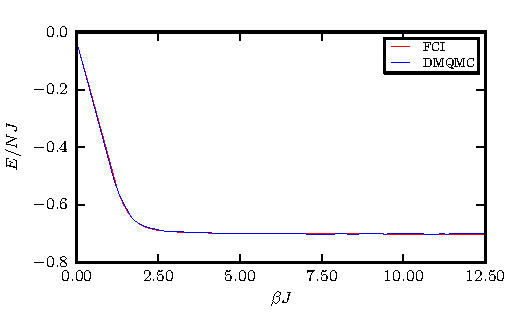
\includegraphics[width =1\textwidth]{4x4_nois_energy.pdf}
\caption[The DMQMC finite-temperature energy estimator for the $4\times4$ antiferromagnetic Heisenberg model.]{The DMQMC finite-temperature energy estimator (blue) and the exact FCI energy (red) for the $4\times4$ antiferromagnetic Heisenberg model. The DMQMC simulation ran with an initial population of $10^5$ psips and for $10^3$ $\beta$-loops. }
\label{fig:4x4_nois_energy}
\end{center}
\end{figure}
\begin{figure}[H]
\begin{center}
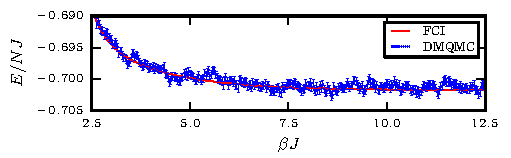
\includegraphics[width =1\textwidth]{4x4_energy_subplot.pdf}
\caption[The DMQMC energy estimator for the $4\times4$ antiferromagnetic Heisenberg model.]{The DMQMC finite-temperature energy estimator with statistical errors (blue) and the exact FCI energy (red) for the $4\times4$ antiferromagnetic Heisenberg model.}
\label{fig:4x4_nois_energy_subplot}
\end{center}
\end{figure}

A blocking analysis over a single $\beta$-loop yields a ground-state energy estimate of $E_0 = -0.7021(3)$, which is within error of the FCI ground-state energy\cite{SpencerFCI} of $E_0 = -0.7018$.

However, the number of psips used was larger than the size of the Hilbert space\footnote{But considerably less than the $1.7\times10^8$ elements of the density matrix}. So whilst the DMQMC results are reasonably accurate, the finite-temperature properties can be calculated with far less effort using FCI. For example, the DMQMC simulation running on 64 cores (2.8 Ghz) took approximately 3 hours to complete, whereas the FCI calculation took approximately 30 minutes on 2 cores (1.86 GHz). This could prove to be a problem with larger systems where even more psips are required.

\subsection{Staggered magnetisation}
The DMQMC finite-temperature squared staggered magnetisation estimator was also tested on the $4\times4$ antiferromagnetic Heisenberg model and the results are presented in Fig.~\ref{fig:4x4_nois_stag_mag} and  Fig.~\ref{fig:4x4_nois_stag_mag_subplot}. A blocking analysis over a single $\beta$-loop yields a ground-state squared staggered magnetisation estimate of $\langle (M^{\dagger})^2\rangle_0 = 0.2762(5)$, which agrees (within error) with the exact result of $\langle (M^{\dagger})^2\rangle_0 = 0.2765$ obtained by Dagotto and Moreo\cite{Dagotto1988} using a modified Lanczos method.
\begin{figure}[H]
\begin{center}
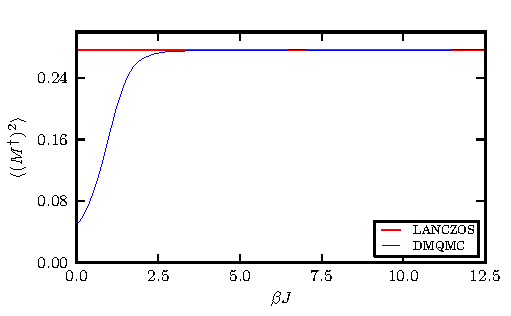
\includegraphics[width =1\textwidth]{4x4_nois_stag_mag.pdf}
\caption[The DMQMC finite-temperature squared staggered magnetisation estimator for the $4\times4$ antiferromagnetic Heisenberg model.]{The DMQMC finite-temperature squared staggered magnetisation estimator (blue) and the exact modified Lanczos ground-state squared staggered magnetisation (red) for the $4\times4$ antiferromagnetic Heisenberg model. The DMQMC simulation ran with an initial population of $10^5$ psips and for $10^3$ $\beta$-loops.}
\label{fig:4x4_nois_stag_mag}
\end{center}
\end{figure}
\begin{figure}[H]
\begin{center}
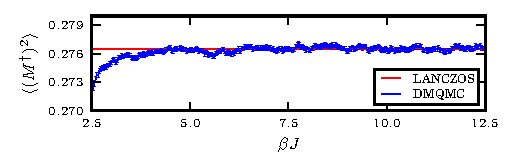
\includegraphics[width =1\textwidth]{4x4_stag_mag_subplot.pdf}
\caption[The DMQMC finite-temperature squared staggered magnetisation estimator with statistical errors for the $4\times4$ antiferromagnetic Heisenberg model.]{The DMQMC finite-temperature squared staggered magnetisation estimator with statistical errors (blue) and the exact modified Lanczos ground-state squared staggered magnetisation (red) for the $4\times4$ antiferromagnetic Heisenberg model.}
\label{fig:4x4_nois_stag_mag_subplot}
\end{center}
\end{figure}


\subsection{Heat capacity}
\label{sec:HeatCapacityResults}
Two methods for calculating the heat capacity in a constant magnetic field were introduced in Sec.~\ref{sec:heatCapacity}. One method was to calculate the derivative in Eq.~\ref{eq:splineDerivative} using a cubic spline fit of the finite-temperature energy estimator and the other was to directly sample the heat capacity during the DMQMC simulation. Both were tested on the $4\times4$ antiferromagnetic Heisenberg lattice with no magnetic field and are shown in Fig.~\ref{fig:4x4spline_spec_heat}. 

\begin{figure}[H]
\begin{center}
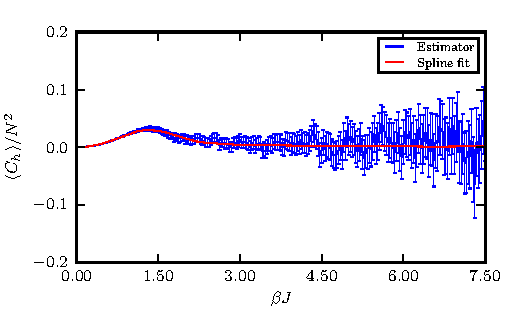
\includegraphics[width =1\textwidth]{4x4spline_spec_heat.pdf}
\caption[The heat capacity estimator calculated by the spline derivative method (red) and by direct stochastic sampling (blue) for a $4\times4$ antiferromagnetic Heisenberg lattice with no applied magnetic field]{The heat capacity estimator calculated by the spline derivative method (red) and by direct stochastic sampling (blue) for a $4\times4$ antiferromagnetic Heisenberg lattice.}
\label{fig:4x4spline_spec_heat}
\end{center}
\end{figure}

It was found that the spline fit method worked best. The direct stochastic sampling of the heat capacity suffered from huge fluctuations as $\beta$ grew large. This is due to the $\beta^2$ factor in Eq.~\ref{eq:heatCapacityEstimator}. As $\beta$ becomes large the fluctuations in $\langle H^2\rangle-\langle H\rangle^2$ are amplified resulting in heavy statistical noise. This is not the case for the other estimators studied, where the factor is absent. The spline fit on the $\langle H \rangle$ estimator smooths out the statistical fluctuations and removes the dependence on the $\langle H^2\rangle$ estimator, so performs better. Furthermore, the spline derivative method tends towards the correct value in the large $\beta$ limit. The heat capacity should be zero at absolute zero otherwise the third law of thermodynamics would be violated

\section{The $6\times6$ antiferromagnetic Heisenberg Lattice}
The Hilbert space of the $6\times6$ antiferromagnetic Heisenberg lattice contains a much larger $9.08\times10^9$ configurations in the $M_S = 0$ subspace. Although it is unfeasible to calculate exact FCI results for this system, it has been well-studied in the literature by methods such as GFQMC.

Fig.~\ref{fig:6x6_no_importance_sampling2_energy} shows the DMQMQ finite-temperature energy estimator fluctuating wildly after only a short range in $\beta$. It was not possible to obtain the ground-state energy. This simulation took roughly 10.5 hours on 64 cores (2.8 Ghz) and although the number of psips was only a fraction of the Hilbert space, DMQMC cannot be regarded as a competitive QMC algorithm unless some major improvements are found.
\begin{figure}[H]
\begin{center}
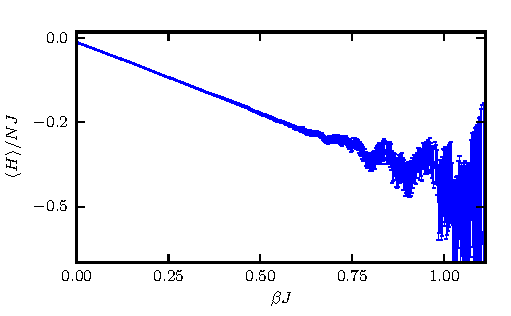
\includegraphics[width =0.82\textwidth]{6x6_no_importance_sampling2_energy.pdf}
\caption[The DMQMC finite-temperature energy estimator for the $6\times6$ antiferromagnetic Heisenberg model. ]{The DMQMC finite-temperature energy estimator for the $6\times6$ antiferromagnetic Heisenberg model.  The simulation ran with an initial population of $10^6$ psips and for $10^3$ $\beta$-loops.}
\label{fig:6x6_no_importance_sampling2_energy}
\end{center}
\end{figure}

\section{Importance sampling}
\label{sec:importanceSampling}

It was soon discovered that DMQMC was ineffective because the number of psips on the diagonal of the density matrix decays exponentially with inverse-temperature as shown in Fig.~\ref{fig:6x6_no_importance_sampling2_trace}. As psips spawn out from the diagonal and start to explore the complete space of density matrix elements, the chance of them spawning back onto the trace becomes very small. For example, psips that carry more than 1 excitation between their bitstring labels can no longer spawn directly back onto the diagonal, but have to do so in a number of steps. Meanwhile, the psips that were originally on the trace are killed off by the clone/death step of the DMQMC algorithm and so the population quickly diminishes. 
\begin{figure}[H]
\begin{center}
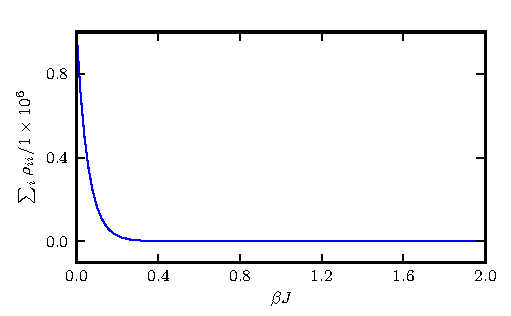
\includegraphics[width =1\textwidth]{6x6_no_importance_sampling2_trace.pdf}
\caption[Total number of psips on the trace as a function of $\beta$.]{Total number of psips on the trace as a function of $\beta$.}
\label{fig:6x6_no_importance_sampling2_trace}
\end{center}
\end{figure}

In order to improve the statistics on the trace at large $\beta$, spawning events onto the diagonal can be encouraged in a way that can be undone when calculating expectation value estimators. This can be achieved by increasing the probability of psips spawning onto the diagonal and assigning them a weight to be taken into account when calculating the estimators. More generally, to improve the statistics across all excitations, psips can either be encouraged or discouraged to spawn from one excitation to another and then assigned the relevant weight.

One can think of a scalar function $\mathcal{M}$, which maps an element of $\bm{\rho}$ to an element of a new matrix $\bm{\rho}'$, which evolves with improved statistics across all excitations. The scalar function takes as its arguments, the configurations $\ket{i}$ and $\ket{j}$ that represent the position of the element in $\bm{\rho}$ and the matrix element $\rho_{ij}$ itself. The function compares the two configurations and determines the number of excitations between them and hence scales the matrix element accordingly (equivalent to scaling the number of psips). So $\mathcal{M}$ can be thought of in the following way,
\begin{equation}
\rho'_{ij} = \mathcal{M}(\rho_{ij},\ket{i},\ket{j}) = W(\ket{i},\ket{j})\rho_{ij},
\label{eq:importanceSamplingTransformation}
\end{equation}
where $W$ is a scalar function that determines the excitation between $\ket{i}$ and $\ket{j}$ and returns the appropriate scaling factor. It is important to note that $W(\ket{i},\ket{j}) = W(\ket{j},\ket{i})$ as $\bm{\rho}$ is symmetric.

Now the inverse of $\mathcal{M}$ is obvious,
\begin{equation}
\mathcal{M}^{-1}(\ket{i},\ket{j},{\rho'}_{ij}) =  \frac{1}{W(\ket{i},\ket{j})}{\rho'}_{ij} = \rho_{ij}
\end{equation}

To make notation simple define
\begin{eqnarray}
\mathcal{M}({\rho}_{ij})  &\equiv& \mathcal{M}(\ket{i},\ket{j},\rho_{ij}) \\
\mathcal{M}^{-1}({\rho'}_{ij})  &\equiv& \mathcal{M}^{-1}(\ket{i},\ket{j},{\rho'}_{ij}) \\
W_{ij} &\equiv& W(\ket{i},\ket{j}).
\end{eqnarray}

Under this transformation the estimator for the expectation value of an operator, $O$, can be written
\begin{eqnarray}
\langle O \rangle = \frac{\sum_{i,j}\rho_{ij}O_{ji}}{\sum_{i}\rho_{ii}} &= & \frac{\sum_{i,j}\mathcal{M}^{-1}({\rho'}_{ij})O_{ji}}{\sum_{i}\mathcal{M}^{-1}({\rho'}_{ii})}\\
&=& \frac{\sum_{i,j}\frac{1}{W_{ij}}{\rho'}_{ij}O_{ji}}{\sum_{i}\mathcal{M}^{-1}({\rho'}_{ii})}\\
&=& W_{ii}\frac{\sum_{i,j}{\rho'}_{ij}\mathcal{M}^{-1}(O_{ji})}{\sum_{i}{\rho'}_{ii}}.
\label{eq:importanceSampledEstimator}
\end{eqnarray}
In the final step $\frac{1}{W_{ij}}O_{ji} = \mathcal{M}^{-1}(O_{ji})$ due to the symmetry of $W$ and the fact that $\bm{O}$ and $\bm{\rho}$ are expressed in the same basis. Moreover, $W_{ii}$ has been taken out of the summation because for each $i$ the excitation level is zero and hence $W_{ii}$ is constant.

So under the importance sampling transformation (Eq.~\ref{eq:importanceSamplingTransformation}), expectation value estimators can be obtained by applying the inverse transformation to the matrix $\bm{O}$, then taking the expectation value with respect to $\bm{\rho}'$ and finally multiplying by the weight given to the zeroth excitation. If the weights $W_{ij}$ are chosen carefully then the statistical error on the expectation value can be minimised.

\subsection{New population dynamics}

Given the importance sampling transformation (Eq.~\ref{eq:importanceSamplingTransformation}) it is possible to deduce a new set of rules for the population dynamics for the evolution of $\bm{\rho}'$, by transforming Eq.~\ref{eq:FirstOrderEuler},
\begin{multline}
\mathcal{M}^{-1}({\rho'}_{ij}(\beta +\Delta \beta)) = \\ \mathcal{M}^{-1}({\rho'}_{ij}(\beta))+\frac{1}{2}\sum_{m}\left(T_{im}\mathcal{M}^{-1}({\rho'}_{mj}(\beta))+\mathcal{M}^{-1}({\rho'}_{im}(\beta))T_{mj}\right)\Delta\beta.
\end{multline}
This simplifies to
\begin{equation}
{\rho'}_{ij}(\beta +\Delta \beta) = {\rho'}_{ij}(\beta)+\frac{1}{2}\sum_{m}\left(\frac{W_{ij}}{W_{mj}}T_{im}{\rho'}_{mj}(\beta)+{\rho'}_{im}(\beta)\frac{W_{ij}}{W_{im}}T_{mj}\right)\Delta\beta
\end{equation}

Therefore the rates at which psips spawn has changed so that they spawn from
\begin{equation}
\label{eq:ImportanceSpawningWeights}
(i,m)\to(i,j) \textnormal{\phantom{---}with probability\phantom{---}} \frac{W_{ij}}{2W_{im}}\lvert T_{mj} \rvert
\end{equation}
and from
\begin{equation}
\label{eq:ImportanceSpawningWeights2}
(m,j)\to(i,j) \textnormal{\phantom{---}with probability\phantom{---}} \frac{W_{ij}}{2W_{mj}}\lvert T_{im} \rvert.
\end{equation}
It is also important to note that when spawning in the opposite direction to in Eq.~\ref{eq:ImportanceSpawningWeights} and Eq.~\ref{eq:ImportanceSpawningWeights2} then the inverse weights must be applied.


\subsection{Choosing the weights}
An optimal set of weights can be chosen by studying the number of psips on each excitation level during a standard DMQMC run. Fig.~\ref{fig:excitations_nois} shows an example how the population of psips on each excitation changes as a function of $\beta$. In the ground-state some excitation levels are poorly sampled because they are occupied by small numbers of psips. 

\begin{figure}[H]
\begin{center}
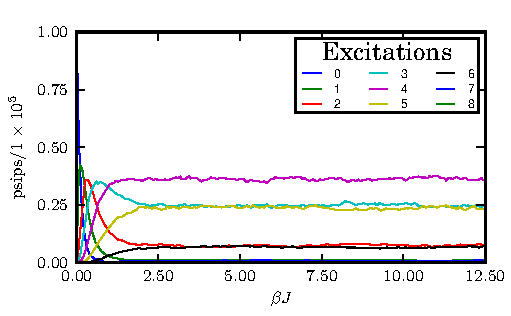
\includegraphics[width =1\textwidth]{excitations_nois.pdf}
\caption[The distribution of psips across the different excitation levels for a single $\beta$-loop of a DMQMC simulation of a $4\times4$ antiferromagnetic Heisenberg lattice.]{The distribution of psips across the different excitation levels for a single $\beta$-loop of a DMQMC simulation of a $4\times4$ antiferromagnetic Heisenberg lattice.}
\label{fig:excitations_nois}
\end{center}
\end{figure}
In the ground-state the number of psips on each excitation remains approximately constant. At this point the weights from Sec.~\ref{sec:importanceSampling} can be determined so that the total population of psips is distributed uniformly over the different excitation levels. For instance,
\begin{equation}
\label{eq:weightSelection}
W_n = \frac{N_{p}^{tot}}{N_{ex}N_p^{n}},
\end{equation}
where $W_n$ is the weight for the $n^{th}$ excitation, $N_p^{tot}$ is the total number of psips across all excitations,  $N_{ex}$ is the total number of excitations and $N_p^{n}$ is the total number of psips on the $n^{th}$ excitation.

When the importance sampling method was first tested, the weights were applied at the start of the simulation as shown in Fig~\ref{fig:excitations_is_instant}. 
\begin{figure}[H]
\begin{center}
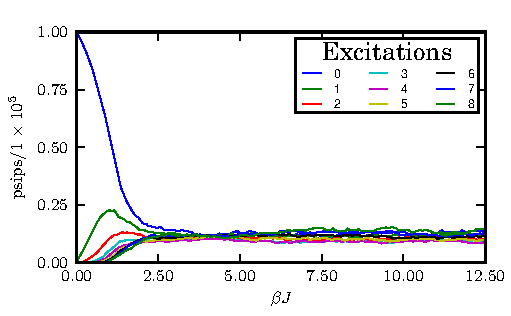
\includegraphics[width =1\textwidth]{excitations_is_instant.pdf}
\caption[The distribution of psips across the different excitation levels for a single $\beta$-loop of a DMQMC simulation of a $4\times4$ antiferromagnetic Heisenberg lattice, with importance sampling weights fully applied at $\beta = 0$.]{The distribution of psips across the different excitation levels for a single $\beta$-loop of a DMQMC simulation of a $4\times4$ antiferromagnetic Heisenberg lattice, with importance sampling weights fully applied at $\beta = 0$.}
\label{fig:excitations_is_instant}
\end{center}
\end{figure} It is evident that initially spawning events from the diagonal are restricted leading to an effective truncation of the Hilbert space as other excitations are suppressed. This meant that the higher excitations were being under-sampled for the initial evolution, which lead to biased results.

The weights were then introduced gradually, as shown in Fig.~\ref{fig:excitations_is}, so that in the ground-state ($\beta > \beta_{gs}$) they had reached the intended values. Each weight, $W$, was set to unity at $\beta = 0$ and for each step of $\Delta \beta$ they were scaled by $W^{\frac{\Delta\beta}{\beta_{gs}}}$ so that for $\beta > \beta_{gs}$ the weights were fully applied. Gradually introducing the weights in this way avoided a discontinuity in the spawning probabilities, whilst also reducing the effective truncation of the Hilbert space.  In this way, the psip populations in the pre-ground-state evolution is more similar to the case where no importance sampling is applied (Fig.~\ref{fig:excitations_nois}).

\begin{figure}[H]
\begin{center}
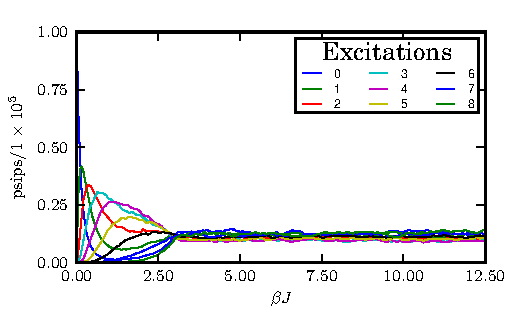
\includegraphics[width =1\textwidth]{excitations_is.pdf}
\caption[The distribution of psips across the different excitation levels for a single $\beta$-loop of a DMQMC simulation of a $4\times4$ antiferromagnetic Heisenberg lattice, with the importance sampling weights introduced gradually.]{The distribution of psips across the different excitation levels for a single $\beta$-loop of a DMQMC simulation of a $4\times4$ antiferromagnetic Heisenberg lattice, with the importance sampling weights introduced gradually. }
\label{fig:excitations_is}
\end{center}
\end{figure}

\subsection{Importance sampling implementation}
This method of importance sampling is simple to implement. When attempting to spawn, as in Eq.~\ref{eq:ImportanceSpawningWeights}, the excitation level of the current density matrix element can be found by performing a bit-wise \texttt{XOR} between the two bistrings that label it. The number of bits that are set in the output is equal to the number of excitations between the two bitstrings. This operation can also be used to determine the number of excitations between the two bitstrings labelling the density matrix element that a psip is spawning to. It is then easy to apply the correct weight to the spawning probability using Eq.~\ref{eq:ImportanceSpawningWeights}.

When adding the contribution from a particular density matrix element to the estimator, the above weighting can be undone easily by calculating the excitation level between the two labelling bit strings (using the bit-wise \texttt{XOR} operation) and then dividing by the corresponding weight.

\section{The $6\times6$ antiferromagnetic Heisenberg lattice revisited}
Now that an importance sampling method has been established, the $6\times6$ antiferromagnetic Heisenberg model can be re-investigated. 
\subsection{Energy}
The importance-sampled DMQMC energy estimator is shown in Fig~\ref{fig:6x6_10000000_6_energy} and with errors in Fig~\ref{fig:6x6_10000000_6_energy_subplot}. It shows a dramatic improvement in performance over standard DMQMC and with considerably less sampling. The energy now converges towards a reasonable value for the ground-state energy. For example, a blocking analysis of the DMQMC energy estimator yielded a ground-state energy of $E_0 = -0.6781(5)$, compared to Runge's GFQMC ground-state energy\cite{Runge1992} of $E_0 = -0.678871(8)$. An interesting point to note is that in this case the initial number of psips occupy only $1.21\times10^{-13}$ of the elements of the density matrix, so the performance improvement is huge.

\subsection{Staggered magnetisation}

The importance-sampled DMQMC squared staggered magnetisation estimator is shown in Fig~\ref{fig:6x6_10000000_6_energy}. The squared staggered magnetisation estimator converges to the ground-state value of $\langle (M^{\dagger})^2\rangle_0 = 0.2098(2)$, which was found via a blocking analysis of a single $\beta$-loop. This agrees with the value of $\langle (M^{\dagger})^2\rangle_0 = 0.20986(8)$ that was calculated by Runge using GFQMC\cite{Runge1992a}.

\begin{figure}[H]
\begin{center}
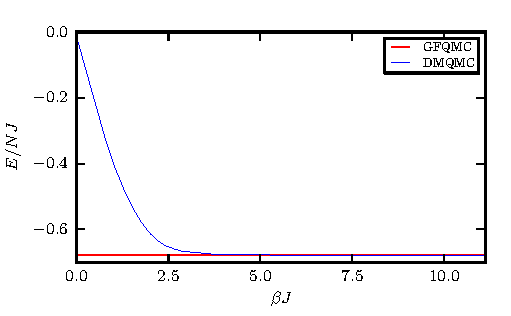
\includegraphics[width =1\textwidth]{6x6_10000000_6_energy.pdf}
\caption[The DMQMC finite-temperature energy estimator with importance sampling for the $6\times6$ antiferromagnetic Heisenberg model]{The DMQMC finite-temperature energy estimator with importance sampling (blue) and an accurate GFQMC estimate for the ground-state energy (red) for the $6\times6$ antiferromagnetic Heisenberg model. The simulation ran with an initial population of $1\times10^7$ psips and for $6$ $\beta$-loops. }
\label{fig:6x6_10000000_6_energy}
\end{center}
\end{figure} 
\begin{figure}[H]
\begin{center}
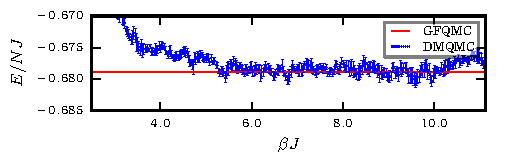
\includegraphics[width =1\textwidth]{6x6_10000000_6_energy_subplot.pdf}
\caption[The importance-sampled DMQMC finite-temperature energy estimator with statistical errors for the $4\times4$ antiferromagnetic Heisenberg model.]{The importance-sampled DMQMC finite-temperature energy estimator with statistical errors (blue) and an accurate GFQMC estimate for the ground-state energy (red) for the $4\times4$ antiferromagnetic Heisenberg model. }
\label{fig:6x6_10000000_6_energy_subplot}
\end{center}
\end{figure}

\begin{figure}[H]
\begin{center}
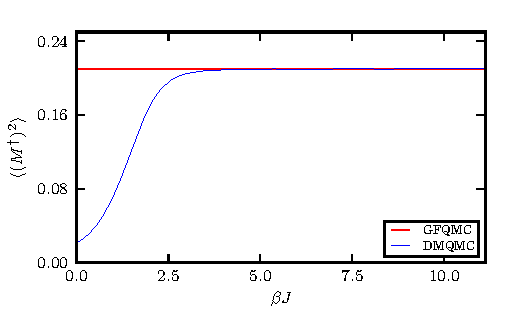
\includegraphics[width =1\textwidth]{6x6_10000000_6_stag_mag.pdf}
\caption[The DMQMC finite-temperature squared staggered magnetisation estimator with importance sampling for the $6\times6$ antiferromagnetic Heisenberg model.]{The DMQMC finite-temperature squared staggered magnetisation estimator with importance sampling (blue) and an accurate GFQMC estimate for the ground-state squared staggered magnetisation (red) for the $6\times6$ antiferromagnetic Heisenberg. The simulation ran with an initial population of $10^7$ psips and for $6$ $\beta$-loops.}
\label{fig:6x6_10000000_6_stag_mag}
\end{center}
\end{figure}
\begin{figure}[H]
\begin{center}
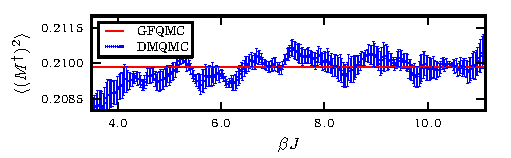
\includegraphics[width =1\textwidth]{6x6_10000000_6_stag_mag_subplot.pdf}
\caption[The importance-sampled DMQMC finite-temperature squared staggered magnetisation estimator with statistical errors or the $6\times6$ antiferromagnetic Heisenberg model.]{The importance-sampled DMQMC finite-temperature squared staggered magnetisation estimator with statistical errors (blue) and an accurate GFQMC estimate for the ground-state square staggered magnetisation (red) for the $6\times6$ antiferromagnetic Heisenberg model. }
\label{fig:6x6_10000000_6_stag_mag_subplot}
\end{center}
\end{figure}
%\subsection{Heat capacity}
%\begin{figure}[H]
%\begin{center}
%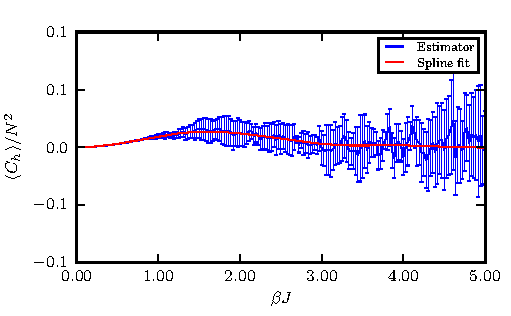
\includegraphics[width =1\textwidth]{6x6spline_spec_heat.pdf}
%\caption{}
%\label{fig:6x6spline_spec_heat}
%\end{center}
%\end{figure}

\section{The $4\times4\times4$ antiferromagnetic Heisenberg lattice}
The importance-sampled DMQMC algorithm was also tested on the $4\times4\times4$ antiferromagnetic Heisenberg lattice and the results are shown in Fig.~\ref{fig:4x4x4_is_energy} and Fig.~\ref{fig:4x4x4_is_energy_subplot}. It was difficult to test the accuracy of the DMQMC method in three dimensions, as the three dimensional antiferromagnetic Heisenberg model features less prominently in the literature. Nevertheless, the DMQMC ground-state energy estimate was compared against an accurate ground-state energy estimate obtained via FCIQMC\cite{SpencerFCIQMC}. 

Performing a blocking analysis, on a single $\beta$-loop DMQMC simulation gives a ground-state energy of $E_0 = -0.912(6)$, whereas a single run of the FCIQMC algorithm\cite{SpencerFCIQMC} gives a ground-state energy of $E_0 = -0.91509(5)$. The FCIQMC value was obtained using an initial population of $10^6$ psips. DMQMC seems a good compromise between accuracy and the ability to obtain finite-temperature estimates.

The Hilbert space for a $4 \times 4 \times 4$ lattice contains roughly $1.83\times10^{18}$ spin configurations and so in this case DMQMC was simulating a density matrix with approximately $1.83\times10^{36}$ elements using only $5\times10^5$ psips. The statistical errors in Fig.~\ref{fig:4x4x4_is_energy_subplot} are surprisingly small considering the number of psips used.

\begin{figure}[H]
\begin{center}
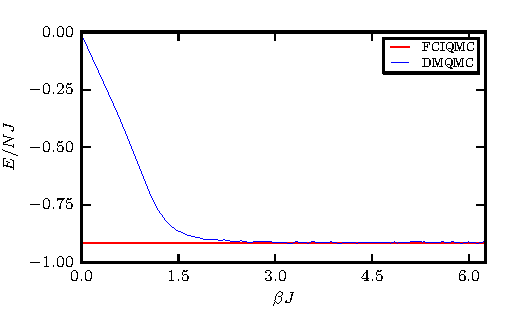
\includegraphics[width =1\textwidth]{4x4x4_is_energy.pdf}
\caption[The DMQMC finite-temperature energy estimator with importance sampling for the $4\times4\times4$ antiferromagnetic Heisenberg model.]{The DMQMC finite-temperature energy estimator with importance sampling (blue) and an accurate FCIQMC estimate for the ground-state energy (red) for the $4\times4\times4$ antiferromagnetic Heisenberg model.  The simulation ran with an initial population of $5\times10^6$ psips and for $43$ $\beta$-loops.}
\label{fig:4x4x4_is_energy}
\end{center}
\end{figure}
\begin{figure}[H]
\begin{center}
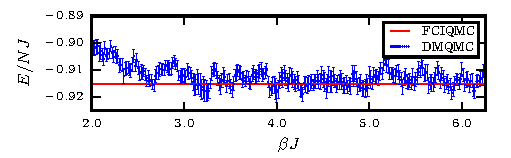
\includegraphics[width =1\textwidth]{4x4x4_is_energy_subplot.pdf}
\caption[The importance-sampled DMQMC finite-temperature energy estimator with statistical errors for the  $4\times4\times4$ antiferromagnetic Heisenberg model.]{The importance-sampled DMQMC finite-temperature energy estimator with statistical errors (blue) and an accurate FCIQMC estimate for the ground-state energy (red) for the $4\times4\times4$ antiferromagnetic Heisenberg model.}
\label{fig:4x4x4_is_energy_subplot}
\end{center}
\end{figure}

\section{Summary}
The DMQMC implementation was tested on some simple antiferromagnetic Heisenberg models in both two and three dimensions. With the standard algorithm, developed in Ch.~\ref{ch:chapter1}, it was found that the initial population of psips was similar to the size of the Hilbert space of configurations and failed for larger systems. It appeared as though the method might not be efficient enough to compete as a QMC method. 

However, the reason for this poor performance was soon realised and a suitable importance sampling adaptation to the algorithm was invented, giving dramatically improved results. This new method allowed for accurate finite-temperature calculations of energy and staggered magnetisation for the $6\times6$ Heisenberg lattice, for which the conventional DMQMC method had failed. Importance sampling also enabled accurate simulation of the $4\times4\times4$ antiferromagnetic Heisenberg model. In most cases the DMQMC ground-state estimators (obtained via a blocking analysis) were equal to the results in the literature, within error.

Additionally, both versions of the heat capacity estimator were tested on the $4\times4$ antiferromagnetic Heisenberg lattice. It was found that directly sampling the heat capacity from the DMQMC simulation gave poor results, even with importance sampling. This was because the statistical fluctuations were amplified for large $\beta$. This proved the point that, although in DMQMC it is theoretically possible to calculate the expectation value of any quantum mechanical operator, in practice it can prove to be difficult to obtain accurate results. The spline derivative method did provide improved results, but this method requires post-processing of the data and makes it difficult to determine errors. 

%%% Local Variables: 
%%% mode: latex
%%% TeX-master: "../thesis"
%%% End: 
